\documentclass[12 pt]{exam}
\usepackage{graphicx, enumitem, amsmath, amssymb}
\graphicspath{ {./images/} }
\usepackage{tikz, pgfplots}
\usetikzlibrary{shapes,arrows}
%\usepackage{Minion Pro}
\printanswers

\title{1.3 Optimization and the Budget Constraint - Practice Problems (Answers)}
\author{Ryan Safner}
\date{ECON 306 - Spring 2020}

\begin{document}

\maketitle
 

You can get music via downloads ($d$) or concert tickets ($t$). You have \$60 to spend each week, and the price of a download is \$3 and the price of a concert ticket is \$10. Put $d$ on the horizontal axis and $t$ on the vertical axis.

\begin{questions}

\question Write the equation for your budget constraint.
	
\begin{solution}
			\begin{equation*}
	m = p_d d + p_t t 	
	\end{equation*}
		\begin{equation*}
	\$60 = \$3d+\$10t	
	\end{equation*}	
		\end{solution}

\question Solve this equation for $t$, to express the equation of the line. 
	\begin{solution}
	Solving for $t$ (on the vertical axis):
\begin{align*}
\$60-\$3d&=\$10t\\
	\frac{\$60}{\$10}-\frac{\$3d}{\$10}&=t\\
	\$6-\frac{\$3}{\$10}d&=t\\
	\end{align*}	
	\end{solution}

\question If you spent all of your money on only Downloads, how many could you buy? If you spent all of your money only on Tickets, how many could you buy? What is the slope of your budget constraint? Graph your budget constraint. 
	\begin{solution}
	Only on Downloads: 
		\begin{equation*}
	\frac{m}{p_d}=\frac{\$60}{\$3}=20	
	\end{equation*}  `
Only on Tickets:
	\begin{equation*}
	\frac{m}{p_t}=\frac{\$60}{\$10}=6	
	\end{equation*}
Graph:\\ 
				\begin{tikzpicture}[xscale=.375, yscale=.75]
			\draw[->] (0,0) -- (22,0) coordinate (x axis) node[right]{$d$};
 			\draw[->] (0,0) -- (0,11) coordinate (y axis) node[above]{$t$};
				\draw[xstep=2cm, ystep=1cm, black, dotted] (0,0) grid (20,10); 
				 				\foreach \x/\xtext in { 0,2,..., 20} 
 					\draw (\x,1pt) -- (\x,-1pt) node[anchor=north] {$\xtext$};
				\foreach \y/\ytext in { 1,..., 10} 
					\draw (1pt,\y) -- (-1pt,\y) node[anchor=east] {$\ytext$};
					\draw[ultra thick, blue](0,6)--(20,0);
 		\end{tikzpicture}
	\end{solution}

\question Now suppose your income temporarily decreases to \$30. Find the new equation of the budget constraint and graph it. 
\begin{solution}

To do this simply, find the new intercepts, and recognize that the slope will not change! 

\begin{equation*}
\frac{m}{p_t}=\frac{30}{10}=3 
\end{equation*}

\begin{equation*}
\frac{m}{p_c}=\frac{30}{3}=10	
\end{equation*}

\begin{equation*}
t=3-\frac{3}{10}d	
\end{equation*}

				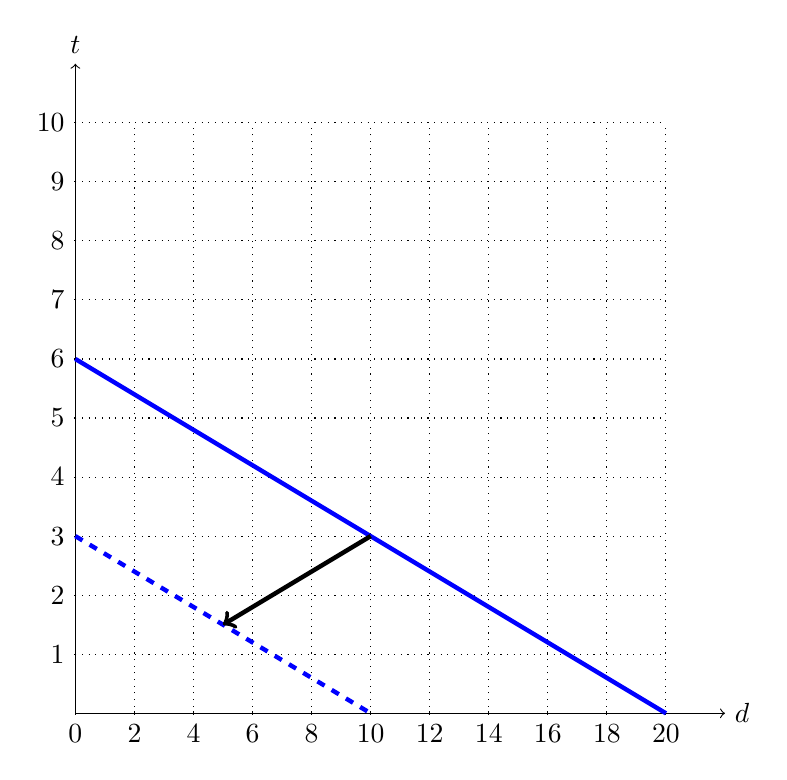
\begin{tikzpicture}[xscale=.375, yscale=.75]
			\draw[->] (0,0) -- (22,0) coordinate (x axis) node[right]{$d$};
 			\draw[->] (0,0) -- (0,11) coordinate (y axis) node[above]{$t$};
				\draw[xstep=2cm, ystep=1cm, black, dotted] (0,0) grid (20,10); 
				 				\foreach \x/\xtext in { 0,2,..., 20} 
 					\draw (\x,1pt) -- (\x,-1pt) node[anchor=north] {$\xtext$};
				\foreach \y/\ytext in { 1,..., 10} 
					\draw (1pt,\y) -- (-1pt,\y) node[anchor=east] {$\ytext$};
					\draw[ultra thick, blue](0,6)--(20,0);
					\draw[ultra thick, dashed, blue](0,3)--(10,0);
					\draw[ultra thick, ->] (10,3)--(5,1.5);
 		\end{tikzpicture}
\end{solution}

\question Now return to your original income (\$60) but suppose the price of downloads increases to \$6. Find the new equation of the budget constraint and graph it. 
 \begin{solution}
 Start by calculating the most downloads you could buy under the new price:
 		\begin{equation*}
	\frac{m}{p_t}=\frac{\$60}{\$6}=10	
	\end{equation*}  
The price of Tickets hasn't changed, so all we do is rotate the graph with this being the new horizontal intercept. 	\\
				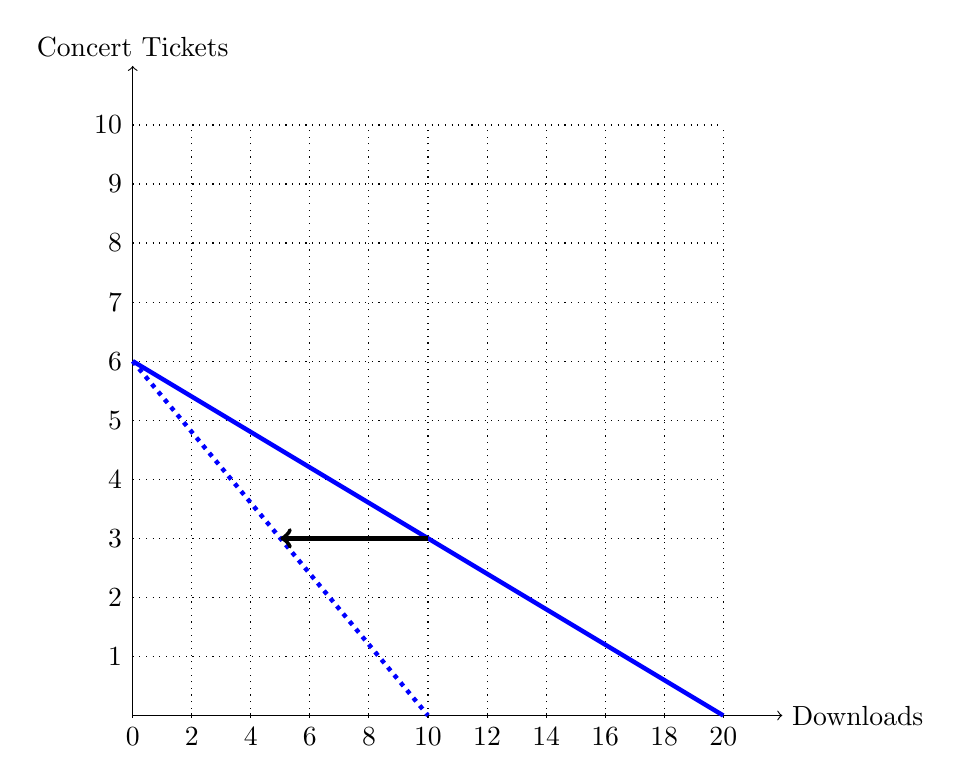
\begin{tikzpicture}[xscale=.375, yscale=.75]
			\draw[->] (0,0) -- (22,0) coordinate (x axis) node[right]{Downloads};
 			\draw[->] (0,0) -- (0,11) coordinate (y axis) node[above]{Concert Tickets};
				\draw[xstep=2cm, ystep=1cm, black, dotted] (0,0) grid (20,10); 
				 				\foreach \x/\xtext in { 0,2,..., 20} 
 					\draw (\x,1pt) -- (\x,-1pt) node[anchor=north] {$\xtext$};
				\foreach \y/\ytext in { 1,..., 10} 
					\draw (1pt,\y) -- (-1pt,\y) node[anchor=east] {$\ytext$};
					\draw[ultra thick, blue](0,6)--(20,0);
					\draw[ultra thick, blue, dotted](0,6)--(10,0);
					\draw[ultra thick, ->](10,3)--(5,3);
 		\end{tikzpicture}
 \end{solution}

\end{questions}
\end{document}